\documentclass[11pt]{amsart}

\usepackage[T1]{fontenc}
\usepackage{lmodern}
\usepackage{amssymb,amsmath}
\usepackage{graphicx}
\usepackage{booktabs}
\usepackage{array}
\usepackage{xcolor}
\usepackage[margin=1.15in]{geometry}
\usepackage[colorlinks=true,linkcolor=blue!50!black,citecolor=blue!50!black,urlcolor=blue!50!black]{hyperref}

\newtheorem{theorem}{Theorem}[section]
\newtheorem{proposition}[theorem]{Proposition}
\newtheorem{lemma}[theorem]{Lemma}
\newtheorem{corollary}[theorem]{Corollary}
\newtheorem*{maintheorem}{Theorem}
\theoremstyle{definition}
\newtheorem{definition}[theorem]{Definition}
\newtheorem{question}[theorem]{Question}
\theoremstyle{remark}
\newtheorem{remark}[theorem]{Remark}

\numberwithin{equation}{section}

\newcommand{\doi}[1]{\href{https://doi.org/#1}{\nolinkurl{doi:#1}}}
\newcommand{\Z}{\mathbb{Z}}
\newcommand{\NN}{\operatorname{N}}
\newcommand{\ind}[1]{[\,#1\,]}
\hypersetup{pdftitle={The book Ramsey number R(B66,B67)},pdfauthor={Deep Bhattacharjee}}

\begin{document}

\title[The book Ramsey number $R(B_{66},B_{67})$]{The book Ramsey number $R(B_{66},B_{67})$}

\author{Deep Bhattacharjee}
\address{Formerly, Electro-Gravitational Space Propulsion Laboratory (EGSPL),\newline Bhubaneswar, Odisha 751030, India}
\email{d.bhattacharjee@erl-forschung.de}
\email{itsdeep@live.com}
\urladdr{https://orcid.org/0000-0003-0466-750X}
\thanks{Corresponding author: \href{mailto:d.bhattacharjee@erl-forschung.de}{d.bhattacharjee@erl-forschung.de}; ORCID \href{https://orcid.org/0000-0003-0466-750X}{\mbox{0000-0003-0466-750X}}}

\subjclass[2020]{Primary 05C55; Secondary 05C25, 05B10}
\keywords{Ramsey number, book graph, block-circulant graph, multiplier group}

\begin{abstract}
We prove that $R(B_{66},B_{67})=267$, the case $n=67$ of Wesley's conjecture $R(B_{n-1},B_n)=4n-1$, which no earlier construction covered. The extremal graph is a two-block circulant graph over $\Z_{133}$ whose connection sets are unions of orbits of the cube roots of unity modulo $133$.
\end{abstract}

\maketitle

\section{Introduction}

The book $B_k$ is the graph $K_2+\overline{K_k}$: $k$ triangles sharing one edge, its spine. For graphs $G$ and $H$, the Ramsey number $R(G,H)$ is the least $N$ such that every graph on $N$ vertices contains $G$ or has a complement containing $H$. Rousseau and Sheehan~\cite{RS} proved, from Goodman's count of monochromatic triangles~\cite{Go}, that
\begin{equation}\label{eq:RS}
R(B_{n-1},B_n)\le 4n-1\qquad(n\ge2).
\end{equation}
Wesley~\cite{We} proved equality for $n\le20$ and whenever $2n-1$ is a prime power congruent to $1$ modulo $4$, and conjectured equality for every $n$. The conjecture is one of the open problems of Epoch AI's FrontierMath collection~\cite{Ep}, which records further progress. Turturean~\cite{Tu} constructed extremal graphs for all $n\le56$ and for fifteen further values below $100$, partly through a cyclotomic construction of Szekeres~\cite{Sz} that applies when $4n-1$ is a prime congruent to $3$ modulo $8$; Chung, Du and Wesley~\cite{CDW} found three further infinite families, from conference graphs, from Legendre pairs and from Yamada--Pott designs; and Price obtained $n=70$~\cite{Ep}.\footnote{The values $n\le100$ that none of the constructions cited here covers are $58$, $59$, $60$, $64$, $65$, $67$, $68$, $72$, $73$, $76$, $78$, $80$, $81$, $84$, $88$, $89$, $92$, $93$, $94$, $96$ and $100$. This list is our reading of~\cite{CDW,Ep,Tu,We} as of 14 October 2026.} The value $n=67$ was not among them. We settle it.

\begin{maintheorem}
$R(B_{66},B_{67})=267$.
\end{maintheorem}

The upper bound is~\eqref{eq:RS}. For the lower bound we exhibit a graph on $266$ vertices with no $B_{66}$ whose complement has no $B_{67}$. It is a two-block circulant graph over $\Z_{133}$, the shape used by Wesley~\cite{We} and Turturean~\cite{Tu}, and its connection sets are invariant under multiplication by the nine cube roots of unity modulo $133$. Section~\ref{sec:blocks} reduces the two book conditions to one inequality~\eqref{eq:star} on the connection sets; the symmetry then reduces~\eqref{eq:star} to ten cases, which Table~\ref{tab:main} records. Every step can be checked by hand, and the graph has also been checked by two independent programs and in Lean~4 (see the end of the paper).

\section{Two-block circulant graphs}\label{sec:blocks}

Throughout, $n\ge2$, $v=2n-1$ and $G=\Z_v$. For $X,Y\subseteq G$ and $d\in G$ put
\[
\NN_{X,Y}(d)=|X\cap(Y+d)|=\#\{y\in Y:\ y+d\in X\}.
\]
Translating by $-d$ shows $\NN_{X,X}(-d)=\NN_{X,X}(d)$, and $\sum_{d\in G}\NN_{X,Y}(d)=|X|\,|Y|$.

Let $A\subseteq G\setminus\{0\}$ with $A=-A$ and $|A|=n-1$, let $C=G\setminus(A\cup\{0\})$, so that $C=-C$ and $|C|=n-1$, and let $B\subseteq G$ with $|B|=n-1$. The graph $\Gamma=\Gamma(A,B)$ has vertex set $G\times\{0,1\}$, and
\[
(x,0)\sim(y,0)\iff y-x\in A,\qquad (x,1)\sim(y,1)\iff y-x\in C,
\]
and $(x,0)\sim(y,1)$ if and only if $y-x\in B$.
Since $A$ and $C$ are symmetric and avoid $0$, $\Gamma$ is a simple graph; in the notation of~\cite{We} it is $\Gamma_G(D_{11},D_{12},D_{22})$ with $D_{11}=A$, $D_{12}=B$, $D_{22}=C$. A vertex $(x,0)$ has $|A|+|B|=2n-2$ neighbours and a vertex $(x,1)$ has $|C|+|B|=2n-2$, so $\Gamma$ is $(2n-2)$-regular on $4n-2$ vertices. The translations $(x,i)\mapsto(x+t,i)$ are automorphisms. Write $\lambda(p,q)$ for the number of common neighbours of two vertices, $\ind{P}$ for the indicator of a statement $P$, and
\[
f(d)=\NN_{A,A}(d)+\NN_{B,B}(d)\qquad(d\in G).
\]

\begin{lemma}\label{lem:lambda}
For $d\ne0$,
\[
\lambda\big((0,0),(d,0)\big)=f(d),\qquad \lambda\big((0,1),(d,1)\big)=f(d)-1+2\ind{d\in A},
\]
and for every $d\in G$, $\lambda\big((0,0),(d,1)\big)=n-1-\ind{d\in B}$.
\end{lemma}

\begin{proof}
A vertex $(z,0)$ is a common neighbour of $(0,0)$ and $(d,0)$ when $z\in A$ and $z-d\in A$, and $(z,1)$ is one when $z\in B$ and $z-d\in B$; this gives $\NN_{A,A}(d)+\NN_{B,B}(d)$.

For $(0,1)$ and $(d,1)$, the common neighbours $(z,1)$ are counted by $\NN_{C,C}(d)$. A vertex $(z,0)$ is adjacent to $(0,1)$ when $-z\in B$ and to $(d,1)$ when $d-z\in B$; with $w=-z$ these say $w\in B$ and $w+d\in B$, so there are $\NN_{B,B}(-d)=\NN_{B,B}(d)$ of them. To compute $\NN_{C,C}(d)$, let $S=A\cup\{0\}$, so $|S|=n$ and $C=G\setminus S$. Then $|C\cap(C+d)|=v-|S\cup(S+d)|=v-2n+|S\cap(S+d)|$. The set $S\cap(S+d)$ is the disjoint union of $A\cap(A+d)$, of $\{0\}$ when $-d\in A$, and of $\{d\}$ when $d\in A$ (neither $0$ nor $d$ lies in $A\cap(A+d)$, because $0\notin A$). As $A=-A$ and $v-2n=-1$, we get $\NN_{C,C}(d)=\NN_{A,A}(d)-1+2\ind{d\in A}$.

For $(0,0)$ and $(d,1)$, a vertex $(z,0)$ is a common neighbour when $z\in A$ and $d-z\in B$, that is, $z=d-b$ with $b\in B$ and $d-b\in A$; since $A=-A$ the last condition reads $b-d\in A$. A vertex $(z,1)$ is a common neighbour when $z\in B$ and $z-d\in C$. Together, $\lambda=\#\{b\in B:\ b-d\in A\cup C\}=\#\{b\in B:\ b\ne d\}=n-1-\ind{d\in B}$.
\end{proof}

\begin{lemma}\label{lem:regular}
In a $(2n-2)$-regular graph on $4n-2$ vertices, two distinct non-adjacent vertices $p,q$ have exactly $\lambda(p,q)$ common non-neighbours other than $p$ and $q$.
\end{lemma}

\begin{proof}
The neighbourhoods of $p$ and $q$ lie in the other $4n-4$ vertices and their union has $2(2n-2)-\lambda(p,q)$ elements; the remaining $\lambda(p,q)$ vertices are adjacent to neither.
\end{proof}

\begin{proposition}\label{prop:star}
$\Gamma(A,B)$ contains no $B_{n-1}$ and its complement contains no $B_n$ if and only if
\begin{equation}\label{eq:star}
f(d)\le n-1-\ind{d\in A}\qquad\text{for every } d\in G\setminus\{0\}.
\end{equation}
In that case $R(B_{n-1},B_n)=4n-1$.
\end{proposition}

\begin{proof}
An edge in $k$ triangles is the spine of a $B_k$. So $\Gamma$ contains no $B_{n-1}$ if and only if every edge has at most $n-2$ common neighbours, and by Lemma~\ref{lem:regular} the complement contains no $B_n$ if and only if every pair of distinct non-adjacent vertices has at most $n-1$ common neighbours. Both conditions together say $\lambda(p,q)\le n-1-\ind{p\sim q}$ for all $p\ne q$, and by translation it suffices to take $p=(0,i)$. We use Lemma~\ref{lem:lambda}. For $p=(0,0)$, $q=(d,1)$ we have $p\sim q$ if and only if $d\in B$, so the condition holds with equality; the pairs $(0,1),(d,0)$ are translates of these. For $p=(0,0)$, $q=(d,0)$ with $d\ne0$ we have $p\sim q$ if and only if $d\in A$, and the condition is~\eqref{eq:star}. For $p=(0,1)$, $q=(d,1)$ we have $p\sim q$ if and only if $d\notin A$, and the condition $f(d)-1+2\ind{d\in A}\le n-2+\ind{d\in A}$ is again~\eqref{eq:star}. The last sentence follows from~\eqref{eq:RS}, since $\Gamma$ has $4n-2$ vertices.
\end{proof}

\begin{remark}\label{rem:slack}
Summing over $d\ne0$ gives $\sum f(d)=2(n-1)(n-2)$ and $\sum\big(n-1-\ind{d\in A}\big)=(n-1)(2n-3)$. So when~\eqref{eq:star} holds, the slacks $s(d)=n-1-\ind{d\in A}-f(d)$ are non-negative integers with sum $n-1$, and~\eqref{eq:star} is an equality for at least $n-1$ of the $2n-2$ values of $d$. The cross edges never matter: $B$ enters only through its autocorrelation $\NN_{B,B}$. For the Paley graphs of~\cite{We} ($v$ a prime power, $A=B$ the nonzero squares), $s=1$ on $A$ and $s=0$ on $C$.
\end{remark}

\begin{lemma}\label{lem:mult}
If $u\in\Z_v^\times$ satisfies $uA=A$ and $uB=B$, then $f(ud)=f(d)$ and $\ind{ud\in A}=\ind{d\in A}$; moreover $f(-d)=f(d)$ and $\ind{-d\in A}=\ind{d\in A}$. Hence, if $H\le\Z_v^\times$ fixes $A$ and $B$, it suffices to check~\eqref{eq:star} for one $d$ in each orbit of the group $\pm H$ on $G\setminus\{0\}$.
\end{lemma}

\begin{proof}
The map $y\mapsto uy$ is a bijection from $X\cap(Y+d)$ onto $uX\cap(uY+ud)$, so $\NN_{uX,uY}(ud)=\NN_{X,Y}(d)$. The statements about $-d$ follow from $\NN_{X,X}(-d)=\NN_{X,X}(d)$ and $A=-A$.
\end{proof}

\section{The case \texorpdfstring{$n=67$}{n = 67}}\label{sec:67}

Let $n=67$ and $v=133=7\cdot19$. Let
\[
H=\{u\in\Z_{133}:u^3=1\}=\{1,11,30,39,58,64,102,106,121\},
\]
the group of cube roots of unity; under $\Z_{133}\cong\Z_7\times\Z_{19}$ it is $\{1,2,4\}\times\{1,7,11\}$. Since $|H|$ is odd, $-1\notin H$ and $\pm H$ has order $18$. Its orbits on $\Z_{133}\setminus\{0\}$ are the following ten: the $108$ units form six orbits of size $18$, with representatives $1,2,3,4,6,8$; on the $18$ nonzero multiples of $7$ the group acts through its image $\pm\{1,7,11\}$ modulo $19$, which has order $6$, giving three orbits, with representatives $7,14,28$; and on the six nonzero multiples of $19$ it acts through its image $\pm\{1,2,4\}=\Z_7^\times$ modulo $7$, giving one orbit, with representative $19$. Put
\begin{align*}
A&=\pm H\cdot\{1,3,4,14,28\},\\
B&=H\cdot\{2,5,8,10,12,14,20,28,57,70\}.
\end{align*}
The first is a union of three orbits of size $18$ and two of size $6$, so $|A|=66$ and $A=-A$; the second is a union of six $H$-orbits of size $9$ and four of size $3$, so $|B|=66$. Explicitly,
\begin{align*}
A=\{&1, 3, 4, 9, 10, 11, 12, 13, 14, 16, 21, 23, 25, 27, 28, 30, 31, 33, 34, 35, 36, 39, 40,\\
&41, 42, 43, 44, 48, 52, 58, 59, 63, 64, 69, 70, 74, 75, 81, 85, 89, 90, 91, 92, 93, 94,\\
&97, 98, 99, 100, 102, 103, 105, 106, 108, 110, 112, 117, 119, 120, 121, 122, 123,\\
&124, 129, 130, 132\},\\
B=\{&2, 5, 8, 10, 12, 13, 14, 17, 18, 20, 21, 22, 24, 26, 27, 28, 31, 34, 37, 42, 45, 46, 48,\\
&50, 54, 55, 57, 60, 62, 63, 65, 68, 69, 70, 71, 73, 75, 78, 79, 83, 87, 88, 89, 91, 94,\\
&95, 96, 98, 103, 105, 107, 108, 109, 110, 111, 113, 114, 115, 116, 122, 124, 125,\\
&128, 129, 131, 132\}.
\end{align*}
The set $B$ is fixed by $H$ but not by $-1$: it meets $-B$ in $42$ elements. Figure~\ref{fig:torus} draws both sets on the torus $\Z_7\times\Z_{19}$.

\begin{figure}[t]
\centering
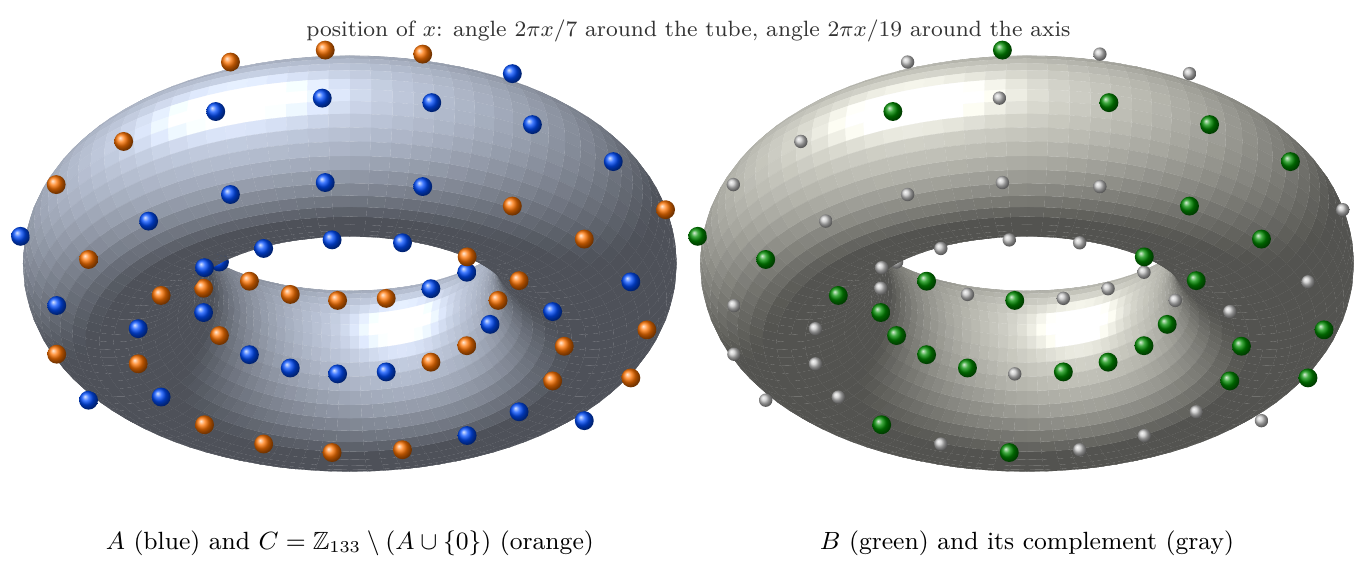
\includegraphics[width=\textwidth]{figures/torus.png}
\caption{The sets $A$ and $B$ for $n=67$. The residue $x\in\Z_{133}$ sits at angle $2\pi x/7$ around the tube and $2\pi x/19$ around the axis, so multiplication by $H=\{1,2,4\}\times\{1,7,11\}$ permutes the points of each picture within its colours.}
\label{fig:torus}
\end{figure}

\begin{table}[t]
\centering
\caption{The inequality~\eqref{eq:star} for $n=67$ on the ten orbits of $\pm H$. The last column is the slack $s(d)$ of Remark~\ref{rem:slack}; the sizes times the slacks add up to $66$.}
\label{tab:main}
\begin{tabular}{r r c r r r r r}
\toprule
$d$ & $|\pm H d|$ & $d\in A$ & $\NN_{A,A}(d)$ & $\NN_{B,B}(d)$ & $f(d)$ & $66-\ind{d\in A}$ & $s(d)$\\
\midrule
 1 & 18 & yes & 36 & 28 & 64 & 65 & 1\\
 2 & 18 & no  & 35 & 31 & 66 & 66 & 0\\
 3 & 18 & yes & 30 & 35 & 65 & 65 & 0\\
 4 & 18 & yes & 32 & 32 & 64 & 65 & 1\\
 6 & 18 & no  & 33 & 33 & 66 & 66 & 0\\
 8 & 18 & no  & 31 & 35 & 66 & 66 & 0\\
 7 &  6 & no  & 33 & 32 & 65 & 66 & 1\\
14 &  6 & yes & 30 & 33 & 63 & 65 & 2\\
28 &  6 & yes & 31 & 34 & 65 & 65 & 0\\
19 &  6 & no  & 30 & 34 & 64 & 66 & 2\\
\bottomrule
\end{tabular}
\end{table}

\begin{theorem}\label{thm:main}
The sets $A$ and $B$ above satisfy~\eqref{eq:star} for $n=67$. Consequently $\Gamma(A,B)$ is a $132$-regular graph on $266$ vertices with no $B_{66}$ whose complement has no $B_{67}$, and $R(B_{66},B_{67})=267$.
\end{theorem}

\begin{proof}
An element $u$ of $H$ fixes $B$, because $B$ is a union of $H$-orbits, and fixes $A$, because $A$ is a union of $\pm H$-orbits. By Lemma~\ref{lem:mult} it suffices to check~\eqref{eq:star} at the ten representatives, and Table~\ref{tab:main} lists $\NN_{A,A}(d)$ and $\NN_{B,B}(d)$ there; each entry is the number of elements of a $66$-element set whose translate by $-d$ stays in the set.\footnote{For instance $\NN_{A,A}(1)=36$ is the number of pairs $a-1,a$ of consecutive residues in $A$: the runs $3,4$; $9,\dots,14$; $27,28$; $30,31$; $33,\dots,36$; $39,\dots,44$; $58,59$; $63,64$; $69,70$; $74,75$; $89,\dots,94$; $97,\dots,100$; $102,103$; $105,106$; $119,\dots,124$; $129,130$ contribute $1+5+1+1+3+5+1+1+1+1+5+3+1+1+5+1=36$.} In every row $f(d)\le66-\ind{d\in A}$. Proposition~\ref{prop:star} gives the rest.
\end{proof}

\begin{figure}[t]
\centering
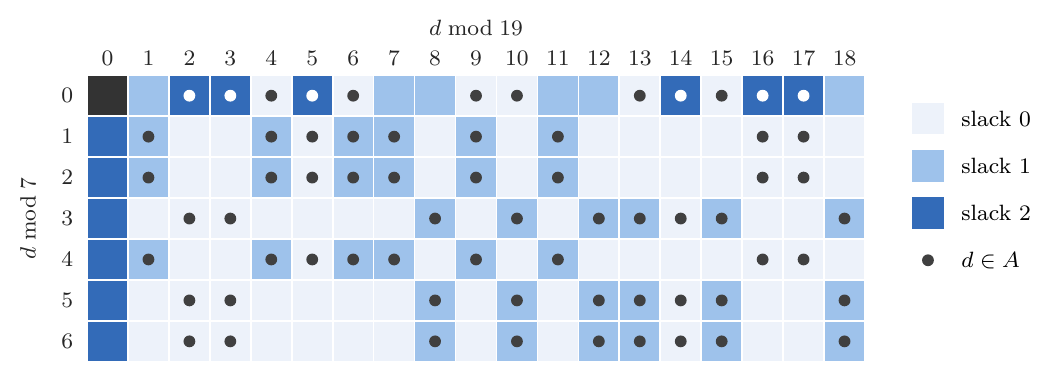
\includegraphics[width=0.92\textwidth]{figures/slack.png}
\caption{The slack $s(d)=66-\ind{d\in A}-f(d)$ for $n=67$ at every $d\ne0$, with $d$ placed by its residues modulo $7$ and $19$; the black cell is $d=0$, and a dot marks $d\in A$. Equality holds for $78$ values of $d$, the slack is $1$ for $42$ and $2$ for $12$.}
\label{fig:slack}
\end{figure}

\section{Remarks}

\begin{remark}
The function $f$ is not constant on $A$ or on $C$ (Figure~\ref{fig:slack}): it takes the values $63$, $64$, $65$ on $A$ and $64$, $65$, $66$ on $C$. So the example is not a difference-set construction of the kind behind the infinite families in~\cite{Sz,Tu,We}, where $f$ is constant on $A$ and on $C$.
\end{remark}

\begin{remark}
The example was found by a computer search. For fixed $v=2n-1$ and a subgroup $H\le\Z_v^\times$, the sets $A$ and $B$ are taken to be unions of $H$-orbits, with $A=-A$; one $0/1$ variable for each orbit in $A$ and one for each orbit in $B$ turn~\eqref{eq:star} into a system of quadratic inequalities, one for each $H$-orbit of $d$, together with $|A|=|B|=n-1$. For $v=133$ the cube roots of unity have $20$ orbits on the nonzero residues, and the CP-SAT solver of OR-Tools~\cite{OR} finds a solution in under a second. The same search did not produce examples for the other values in the footnote to the introduction, for the subgroups and the time limits we tried; some of these systems are infeasible. No step of the proof above depends on the search.
\end{remark}

\begin{question}
Is there an infinite family of two-block circulant graphs, with connection sets invariant under a large multiplier group but $f$ not constant on $A$, that settles further cases of $R(B_{n-1},B_n)=4n-1$? The smallest open case is now $n=58$, with $v=115$.
\end{question}

\subsection*{Formal verification}
Theorem~\ref{thm:main} is also proved in Lean~4~\cite{MU}, without any library beyond the Lean core. The development defines the graph $\Gamma(A,B)$ on the vertices $0,\dots,265$ by the two bit masks of $A$ and $B$, and the kernel evaluates the common neighbours and common non-neighbours of all $35{,}245$ pairs of vertices and checks that the adjacency is symmetric. The final theorem states that every edge has at most $65$ common neighbours and every pair of distinct non-adjacent vertices has at most $66$ common non-neighbours, and it depends only on the standard axioms \texttt{propext}, \texttt{Classical.choice} and \texttt{Quot.sound}. The graph is also checked by two independent programs, in Python and in C, which read the sets $A$ and $B$ and test all pairs directly. The development, the programs and the search are archived in~\cite{Ar}.

\subsection*{Use of generative AI}
The author used Claude (Anthropic) to search for the example, to check it by computer and in Lean, and to draft the text; the author verified every step and is responsible for the content.

\begin{thebibliography}{99}

\bibitem{Ar}
D.~Bhattacharjee, \emph{The book Ramsey number $R(B_{66},B_{67})$: data, checks, search and Lean~4 proof}, 2026. \url{https://github.com/creelie/Breakthrough-problems-2}

\bibitem{CDW}
S.~Chung, W.~Du and W.~J.~Wesley, \emph{Autonomous mathematical discovery in an open-world multi-agent environment}, preprint, 2026. \href{https://arxiv.org/abs/2608.23691}{arXiv:2608.23691}

\bibitem{Ep}
Epoch AI, \emph{FrontierMath open problems: Ramsey numbers for book graphs}, 2026. \url{https://epoch.ai/frontiermath/open-problems/ramsey-book-graphs}, accessed 14 October 2026.

\bibitem{Go}
A.~W.~Goodman, \emph{On sets of acquaintances and strangers at any party}, Amer. Math. Monthly \textbf{66} (1959), no.~9, 778--783. \doi{10.1080/00029890.1959.11989408}

\bibitem{MU}
L.~de~Moura and S.~Ullrich, \emph{The Lean~4 theorem prover and programming language}, in: Automated Deduction -- CADE~28, Lecture Notes in Comput. Sci. \textbf{12699}, Springer, Cham, 2021, 625--635. \doi{10.1007/978-3-030-79876-5_37}

\bibitem{OR}
L.~Perron and F.~Didier, \emph{CP-SAT}, OR-Tools version~9.15, Google, 2025. \url{https://developers.google.com/optimization/cp/cp_solver}

\bibitem{RS}
C.~C.~Rousseau and J.~Sheehan, \emph{On Ramsey numbers for books}, J. Graph Theory \textbf{2} (1978), 77--87. \doi{10.1002/jgt.3190020110}

\bibitem{Sz}
G.~Szekeres, \emph{Tournaments and Hadamard matrices}, Enseign. Math.~(2) \textbf{15} (1969), 269--278.

\bibitem{Tu}
D.~Turturean, \emph{Summary of new results on the Ramsey numbers for book graphs open problem}, 2026. \url{https://docs.google.com/document/d/1VinXOiMov2v-Y27GTJwoAECywv2a34MH4E8qa712zJY}

\bibitem{We}
W.~J.~Wesley, \emph{Lower bounds for book Ramsey numbers}, Discrete Math. \textbf{349} (2026), no.~5, 114913. \doi{10.1016/j.disc.2025.114913}

\end{thebibliography}

\end{document}
